%% LaTeX-Beamer template for KIT design
%% by Erik Burger, Christian Hammer
%% title picture by Klaus Krogmann
%%
%% version 2.1
%%
%% mostly compatible to KIT corporate design v2.0
%% http://intranet.kit.edu/gestaltungsrichtlinien.php
%%
%% Problems, bugs and comments to
%% burger@kit.edu

\documentclass[18pt]{beamer}

%% SLIDE FORMAT

% use 'beamerthemekit' for standard 4:3 ratio
% for widescreen slides (16:9), use 'beamerthemekitwide'


\usepackage{templates/beamerthemekit}
% \usepackage{templates/beamerthemekitwide}

%% TITLE PICTURE

% if a custom picture is to be used on the title page, copy it into the 'logos'
% directory, in the line below, replace 'mypicture' with the 
% filename (without extension) and uncomment the following line
% (picture proportions: 63 : 20 for standard, 169 : 40 for wide
% *.eps format if you use latex+dvips+ps2pdf, 
% *.jpg/*.png/*.pdf if you use pdflatex)

%% Define some colors:
\definecolor{darkblue}{rgb}{0,0,.5}
\definecolor{darkgreen}{rgb}{0,.5,0}

\titleimage{banner}

%% TITLE LOGO

% for a custom logo on the front page, copy your file into the 'logos'
% directory, insert the filename in the line below and uncomment it

\titlelogo{logo_150x150}

% (*.eps format if you use latex+dvips+ps2pdf,
% *.jpg/*.png/*.pdf if you use pdflatex)

%% TikZ INTEGRATION

% use these packages for PCM symbols and UML classes
% \usepackage{templates/tikzkit}
% \usepackage{templates/tikzuml}

% the presentation starts here

\title[Einf\"uhrung]{Tutorium 1}
\subtitle{Einf\"uhrung}
\author{Dominik Muth - dominik.muth@student.kit.edu}

\institute{Institut f\"ur Informatik}

% Bibliography

\usepackage[citestyle=authoryear,bibstyle=numeric,hyperref,backend=biber]{biblatex}
\addbibresource{templates/example.bib}
\bibhang1em

\begin{document}

% change the following line to "ngerman" for German style date and logos
\selectlanguage{ngerman}

%title page
\begin{frame}
	\titlepage
\end{frame}

%table of contents
\begin{frame}{Outline/Gliederung}
	\tableofcontents
\end{frame}

\section{\"Uber Mich}
	\begin{frame}{\"Uber Mich}
		\begin{itemize}
			\item Name: \cite{Dominik Muth} %\language
			\item Studiengang: \cite{Informatik} %\language
			\item E-Mail: \cite{dominik.muth@student.kit.edu} %\language
		\end{itemize}
	\end{frame}

\section{GBI, was ist das?}
	\begin{frame}{GBI}
		\begin{itemize}
			\item Logik
			\pause
			\item Sprachen/Grammatiken
			\pause
			\item Relationen/Abbildungen
			\pause
			\item Graphen
			\pause
			\item Laufzeitabsch\"atzung
			\pause
			\item Automaten
			\pause
			\item Turingmaschinen
			\item \dots
		\end{itemize}
	\end{frame}


\section{Organisatorisches}
\subsection{Allgemeines}
	\begin{frame}{Termine}
		\begin{itemize}
			\item Vorlesung: Mi. 11:30 Uhr im Audimax
			\item \"Ubung: Fr. 9:45 Uhr im Audimax
			\item Klausur: in der Regel anfang M\"arz
		\end{itemize}
	\end{frame}


	\begin{frame}{Links}
		\begin{block}{Vorlesung}
			\begin{itemize}
				\item Website: http://gbi.ira.uka.de
				\item Dozentin: tanja.schultz@kit.edu
			\end{itemize}
		\end{block}

		\begin{block}{Fachschaft}
			\begin{itemize}
				\item Website: http://www.fsmi.uni-karlsruhe.de/
				\item Forum: http://www.fsmi.uni-karlsruhe.de/forum/
			\end{itemize}
		\end{block}
	\end{frame}


\subsection{\"Ubungsbl\"atter}
	\begin{frame}{\"Ubungsbl\"atter}
		\begin{itemize}
			\item Abgabe: Freitag 12:30 Uhr im UG des Infobaus (gegen\"uber der Toiletten) (fr\"uhere Abgabe ist m\"oglich)
			\item 50\% der Punkte zum bestehen n\"otig
		\end{itemize}

		\begin{exampleblock}{must have:}
			\begin{itemize}
				\item Handgeschrieben
				\item Deckblatt
				\item keine Plagiate
			\end{itemize}
		\end{exampleblock}
	\end{frame}


\section{Mengenlehre}
	\begin{frame}{Mengenlehre}

		\begin{block} {Definition Menge}
			Eine Menge ist eine \underline{beliebig} gro\ss{}e Ansammlung an Elementen\\
			$\Rightarrow$ es existieren Mengen ohne, endlich vielen und unendlich vielen Elementen.
		\end{block}

		\begin{block}{Schreibwei\ss{}e von Mengen}
			Sei $M$ eine Menge bestehend aus den Elementen $0, 1, 2$, dann schreiben wir:\\
			\underline{$M = \{0, 1, 2\}$}
			\vspace{10pt}

			Au\ss{}erdem gilt: $0, 1, 2 \in M$

		\end{block}

	\end{frame}



	\begin{frame} {Mengenlehre - Besonderheiten}

		\begin{itemize}
			\item Die Reihenfolge der Elemente in einer Menge ist egal.\\
				Da $x,y \in \{x,y\}$ aber auch $x,y \in \{y,x\}$\\
				$\Rightarrow \{x,y\} = \{y,x\}$
			\pause
			\item Mehrfaches Vorkommen von Elementen ist auch egal.\\
				$\Rightarrow \{a, b, b, 3\} = \{a, b, 3\}$
	
		\end{itemize}
	\end{frame}


	\begin{frame} {Mengenlehre - Besondere Mengen}
		\begin{itemize}
			\item Die Leere Menge: $\emptyset = \{\}$
			\pause
			\item Die Nat\"urlichen Zahlen ohne 0: $\mathbb{N}_+ = \{1,2,3,...\}$
			\pause
			\item Die Nat\"urlichen Zahlen mit 0: $\mathbb{N}_0 = \{0,1,2,3,...\}$
			\pause
			\item Ganze Zahlen von 0 bis n-1: $\mathbb{G}_n = \{0,1,2,...,n-1\}$
		\end{itemize}
	\end{frame}




	\begin{frame}{Mengenoperationen}
		\begin{block}{Vereinigung von Mengen $\cup$}
			Sei $A = \{0,1,2\}$ und $B = \{a,b,c\}$\\
			Dann ist die Vereinigung der Mengen $A$ und $B$:\\
			$A \cup B = \{0,1,2\} \cup \{a,b,c\} = \{0,1,2,a,b,c\}$\\
			Alle Elemente aus $A$ und $B$ liegen somit in $A \cup B$

		\end{block}
		\pause

		\begin{block}{Durchschnitt von Mengen $\cap$}
			Sei $A = \{0,1,2\}$ und $B = \{1,2,3,4,a\}$\\
			Dann ist der Durchschnitt der Mengen $A$ und $B$:\\
			$A \cap B = \{0,1,2\} \cap \{1,2,3,4,a\} = \{1, 2\}$\\
			Im Durchschnitt liegen somit nur Elemente, die sowohl in $A$ und in $B$ liegen.

		\end{block}

	\end{frame}



	\begin{frame}{Aufgabenteil 1}

		Gegeben seien die Mengen $A$, $B$, $C$ und $D$, mit:\\
		$A = \{1,3,5,9\}$\\
		$B = \{1,2,4,8\}$\\
		$C = \{x,d,1,2,3,4,9\}$\\
		$D = \{a,c,d,x\}$
		\vspace{10pt}
		
		Die Menge $M$ sei definiert durch:\\
		\[
			M = \Big(\big(D \cap C\big)\cup\big((C \cap B)\cup(A \cap C)\big)\Big) \setminus (A \cap B)
		\]
		
		Welche Elemente enth\"alt die Menge M?
		\vspace{10pt}	
			
		Antwort: 
		\visible<2>{\color{darkgreen}$M= \{d,x,2,3,4,9\}$}
		%\begin{overprint} 
		%	\onslide<1>
		%		Antwort: \color{white}$M= \{d,x,2,3,4,9\}$
		%	\onslide<2>
		%		Antwort: \color{darkgreen}$M= \{d,x,2,3,4,9\}$
		%\end{overprint}
 	\end{frame}
 	
 	
 	
 	\begin{frame} {Mengenraten}
 	
 	\begin{center}
 	
 		\begin{tabular}{c|c}
 		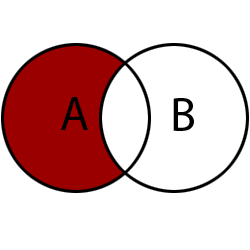
\includegraphics[scale=.35]{graphics/01/menge1.png} &
		\visible<2-4>{
\includegraphics[scale=.35]{graphics/01/menge2.png}}
 		 \\
 		\hline 
 		
 		\visible<3-4>{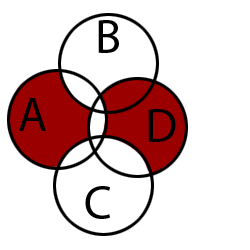
\includegraphics[scale=.35]{graphics/01/menge3.png}}
 		 & 		
 		\visible<4>{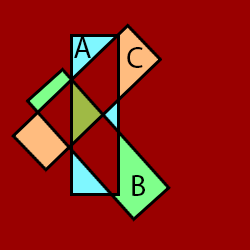
\includegraphics[scale=.35]{graphics/01/menge4.png}} 			\\
 		\end{tabular} 
 		
 		 
		
 	\end{center}
 	
 	\end{frame}


\section{Relationen}
	\begin{frame}{Relationen \\ - Allgemein}

		\begin{block} {Definition Kartesisches Produkt}
			Das Kartesisches Produkt $A \times B$ enth\"allt alle Kombinationen (a,b) mit $a \in A$ und $b \in B$.
		\end{block}
		
		\pause

		\begin{block} {Definition Relation}
			$R \subseteq A \times B$:\\
			Eine Relation ist die Teilmenge eines Kartesischen Produktes.\\
			Andere Schreibweise: $xRy$, mit $(x, y) \in R$
		\end{block}
	\end{frame}



	\begin{frame}{Besonderheiten}
		\begin{block}{Linkstotal}
			Eine Relation ist linkstotal wenn gilt:\\
			f\"ur jedes $a$ existiert \textit{mindestens} ein $b$ f\"ur welches gilt $(a, b) \in R$
		\end{block}
		
		\pause

		\begin{block}{Rechtseindeutig}
			Eine Relation ist rechtseindeutig wenn gilt:\\
			f\"ur kein $a$ existiert mehr als ein $b$ mit $(a, b) \in R$
		\end{block}
		
		\pause

		\begin{block}{}
			Eine Relation, welche sowohl linkstotal als auch rechtseindeutig ist, nennt man auch Abbildung oder Funktion
		\end{block}
	\end{frame}



	\begin{frame}{Besonderheiten}
		\begin{block}{Rechtstotal}
			Eine Relation ist rechtstotal wenn gilt:\\
			f\"ur jedes $b$ existiert \textit{mindestens} ein $a$ f\"ur welches gilt $(a, b) \in R$\\
			rechtstotal $=$ surjektiv
		\end{block}
		
		\pause

		\begin{block}{Linkseindeutig}
			Eine Relation ist linkseindeutig wenn gilt:\\
			f\"ur kein $b$ existiert mehr als ein $a$ mit $(a, b) \in R$\\
			linkseindeutig $=$ injektiv
		\end{block}
		
		\pause

		\begin{block}{}
			Eine surjektive und injektive Relation nennt man bijektiv
		\end{block}
	\end{frame}



	\begin{frame}{Aufgabenteil 2}

		Vervollst\"andige folgende Tabelle, wobei gilt:
		$x \in \mathbb{R}$ und $f(x) \in \mathbb{R}$\\

		\begin{block}{}
			\begin{tabular}{llll}
				\hline
				\textbf{rechtstotal} & \textbf{linkseindeutig} & \textbf{Begriff} & \textbf{Abbildung} \\
				\hline
				? & ? & ? & $f(x) = x^3-x$\\
				? & ? & ? & $f(x) = x^2$\\
				? & ? & ? & $f(x) = x^5$\\
				? & ? & ? & $f(x) = e^{x}$\\
				\hline
			\end{tabular}
		\end{block}

		\pause
		Wie ver\"andert sich die Tabelle, wenn $x \in \mathbb{N}$ und $f(x) \in \mathbb{N}$?
	\end{frame}



	\begin{frame}{Aufgabenteil 2}

		\begin{block}{}
			Gilt f\"ur alle Mengen $M$, dass jede injektive Abbildung $\mathfrak{f} : M \rightarrow M$ auch surjektiv ist?
		\end{block}
			\visible<2>{
				\color{red}Nein: \\
				\color{black} Gegenbeispiel: $M = \mathbb{N}_0$\\
				$ f: n \rightarrow n+1 $}

	\end{frame}
	


	\begin{frame} {EOF}
		\begin{center}
			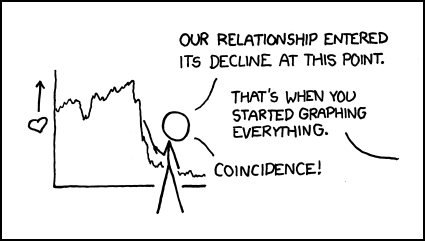
\includegraphics[scale=0.5]{graphics/01/eof1.png}\\
			\tiny source: http://imgs.xkcd.com/comics/decline.png
		\end{center}
	\end{frame}

\end{document}
